\ifx\wholebook\relax \else
% ------------------------

\documentclass[b5paper]{ctexart}
\usepackage[nomarginpar
  %, margin=.5in
]{geometry}

\addtolength{\oddsidemargin}{-0.05in}
\addtolength{\evensidemargin}{-0.05in}
\addtolength{\textwidth}{0.1in}

\usepackage[cn]{../../../prelude}

\setcounter{page}{1}

\begin{document}

\title{红黑树的命令式删除算法}

\author{刘新宇
\thanks{{\bfseries 刘新宇} \newline
  Email: liuxinyu99@hotmail.com \newline}
  }

\maketitle
\fi

\markboth{红黑树}{基本算法}

\ifx\wholebook\relax
\chapter{红黑树的命令式删除算法}
\numberwithin{Exercise}{chapter}
\fi

\index{红黑树!命令式删除}

和插入相比,红黑树的命令式删除算法需要处理更多的情况。在普通二叉搜索树的删除算法之上,我们通过旋转和重新染色恢复平衡性。删除黑色节点会破坏红黑树的第五条性质,使得某一路径上的黑色节点数目减少。为此,我们引入“双重黑色”,来保持黑色节点数目不变。下面的例子程序增加了双重黑色的定义:

\index{红黑树!双重黑色}

\lstset{frame = single}
\begin{lstlisting}[language = Bourbaki]
data Color {RED, BLACK, DOUBLY_BLACK}
\end{lstlisting}

我们首先复用二叉搜索树的删除算法,并记录被删除节点的父节点。如果被删除节点的颜色是黑色,我们通过双重黑色保持性质5,然后再做进一步修复。

\begin{algorithmic}[1]
\Function{Delete}{$T, x$}
  \State $p \gets$ \Call{Parent}{$x$}
  \State $q \gets$ NIL
  \If{\Call{Left}{$x$} = NIL}
    \State $q \gets$ \Call{Right}{$x$}
    \State \textproc{Replace}($x$, \Call{Right}{$x$}) \Comment{用右子树替换$x$}
  \ElsIf{\Call{Right}{$x$} = NIL}
    \State $q \gets$ \Call{Left}{$x$}
    \State \textproc{Replace}($x$, \Call{Left{$x$}}) \Comment{用左子树替换$x$}
  \Else
    \State $y \gets$ \textproc{Min}(\Call{Right}{$x$})
    \State $p \gets$ \Call{Parent}{$y$}
    \State $q \gets$ \Call{Right}{$y$}
    \State \Call{Key}{$x$} $\gets$ \Call{Key}{$y$}
    \State copy data from $y$ to $x$
    \State \textproc{Replace}($y$, \Call{Right}{$y$}) \Comment{用右子树替换$y$}
    \State $x \gets y$
  \EndIf
  \If{\Call{Color}{$x$} = BLACK}
    \State $T \gets$ \textproc{Delete-Fix}($T$, \Call{Make-Black}{$p$, $q$}, $q$ = NIL?)
  \EndIf
  \State release $x$
  \State \Return $T$
\EndFunction
\end{algorithmic}

删除算法接受两个输入:根节点$T$和待删除节点$x$。$x$可以通过查找定位到。如果$x$含有为空的子树,我们将$x$“切下”,并用另一子树$q$来替代$x$。否则,我们在$x$的右子树中找到最小元素$y$,用$y$替换$x$。然后递归地将$y$“切下”。如果$x$是黑色的,我们调用\textproc{Make-Black}($p$, $q$)保持黑色属性,以便进行下一步的修复。

\begin{algorithmic}[1]
\Function{Make-Black}{$p$, $q$}
  \If{$p$ = NIL and $q$ = NIL}
    \State \Return NIL \Comment{树中只有一个叶子节点}
  \ElsIf{$q$ = NIL}
    \State $n \gets$ Doubly Black NIL
    \State \Call{Parent}{$n$} $\gets p$
    \State \Return $n$
  \Else
    \State \Return \Call{Blacken}{$q$}
  \EndIf
\EndFunction
\end{algorithmic}

如果$p$和$q$都为空,我们在删除只有一个叶子节点的树,树变为空。如果父节点$p$不为空,而$q$为空,说明删除了一个黑色叶子节点。我们用NIL替换掉它。根据红黑树性质3,NIL是黑色的。我们把这一NIL变成“双重黑色”的NIL来保持性质5仍然成立。如果$p$、$q$都不为空,我们调用\textproc{Blacken}($q$)检查$q$的颜色,如果是红色的,将它染成黑色,如果$q$已经是黑色的,将它染成双重黑色。接下来,我们通过旋转和重新染色,最终去掉“双重黑色”。这里有三种情况需要处理(\cite{CLRS},292页)。每种情况中,双重黑色的节点即可以是普通节点,也可以是双重黑色NIL。

\textbf{情况1}: {\em 双重黑色节点的兄弟为黑色,并且该兄弟节点有一个红色子节点。}我们可以通过旋转来修复。共有四种细分情况,它们全部可以变换到一种统一形式。如图\cref{fig:del-case1}所示。

\begin{figure}[htbp]
   \centering
   \includegraphics[scale=0.4, page=3]{../../../datastruct/tree/red-black-tree/img/rbtree}
   \caption{双重黑色节点的兄弟为黑色,并且该兄弟节点有一个红色子节点。通过一次旋转操作修复。}
   \label{fig:del-case1}
\end{figure}

\begin{algorithmic}[1]
\Function{Delete-Fix}{$T$, $x$, $f$}
  \State $n \gets$ NIL
  \If{$f$ = True}  \Comment{$x$是双重黑色NIL}
    \State $n \gets x$
  \EndIf
  \If{$x$ = NIL} \Comment{删除唯一的叶子}
    \State \Return NIL
  \EndIf
  \While{$x \neq T$ and \Call{Color}{$x$} $= \mathcal{B}^2$}
    \Comment{$x$是双重黑色,但不是根节点}
    \If{\Call{Sibling}{$x$} $\neq$ NIL} \Comment{兄弟节点不为空}
        \State $s \gets$ \Call{Sibling}{$x$}
        \State ...
        \If{$s$ is black and \Call{Left}{$s$} is red}
          %\Comment{sibling: black, nephew: red}
          \If{$x = $ \textproc{Left}(\Call{Parent}{$x$})}
            \Comment{$x$在左侧}
            \State set $x$, \Call{Parent}{$x$}, and \Call{Left}{$s$} all black
            \State $T \gets$ \Call{Rotate-Right}{$T$, $s$}
            \State $T \gets$ \textproc{Rotate-Left}($T$, \Call{Parent}{$x$})
          \Else \Comment{$x$在右侧}
            \State set $x$, \Call{Parent}{$x$}, $s$, and \Call{Left}{$s$} all black
            \State $T \gets$ \textproc{Rotate-Right}($T$, \Call{Parent}{$x$})
          \EndIf
        \ElsIf{$s$ is black and \Call{Right}{$s$} is red}
          %\Comment{sibling: black, nephew: red}
          \If{$x = $ \textproc{Left}(\Call{Parent}{$x$})} \Comment{$x$在左侧}
            \State set $x$, \Call{Parent}{$x$}, $s$, and \Call{Right}{$s$} all black
            \State $T \gets$ \textproc{Rotate-Left}($T$, \Call{Parent}{$x$})
          \Else \Comment{$x$在右侧}
            \State set $x$, \Call{Parent}{$x$}, and \Call{Right}{$s$} all black
            \State $T \gets$ \Call{Rotate-Left}{$T$, $s$}
            \State $T \gets$ \textproc{Rotate-Right}($T$, \Call{Parent}{$x$})
          \EndIf
        \State ...
        \EndIf
    \EndIf
  \EndWhile
\EndFunction
\end{algorithmic}

\textbf{情况2}: {\em 双重黑色节点的兄弟节点为红色。}可以通过旋转,将双重黑色恢复为普通黑色。如图\cref{fig:del-case2}所示,$a$或$c$恢复为黑色。

\begin{figure}[htbp]
  \centering
  \includegraphics[scale=0.4, page=4]{../../../datastruct/tree/red-black-tree/img/rbtree}
  \caption{双重黑色节点的兄弟节点为红色}
  \label{fig:del-case2}
\end{figure}

我们在此前给出算法上增加这一处理。

\begin{algorithmic}[1]
\Function{Delete-Fix}{$T$, $x$, $f$}
  \State $n \gets$ NIL
  \If{$f$ = True}  \Comment{$x$是双重黑色NIL}
    \State $n \gets x$
  \EndIf
  \If{$x$ = NIL} \Comment{删除唯一的叶子}
    \State \Return NIL
  \EndIf
  \While{$x \neq T$ and \Call{Color}{$x$} $= \mathcal{B}^2$}
    %\Comment{$x$ isn't root and is doubly black}
    \If{\Call{Sibling}{$x$} $\neq$ NIL}
        \State $s \gets$ \Call{Sibling}{$x$}
        \If{$s$ is red}   \Comment{兄弟节点为红色}
          \State set \Call{Parent}{$x$} red
          \State set $s$ black
          \If{$x = $ \textproc{Left}(\Call{Parent}{$x$})} \Comment{$x$在左侧}
            \State $T \gets$ \textproc{Rotate-Left}{$T$, \Call{Parent}{$x$}}
          \Else \Comment{$x$在右侧}
            \State $T \gets$ \textproc{Rotate-Right}{$T$, \Call{Parent}{$x$}}
          \EndIf
        \ElsIf{$s$ is black and \Call{Left}{$s$} is red}
          %\Comment{The sibling is black, a nephew is red}
          \State ...
        \EndIf
    \EndIf
  \EndWhile
\EndFunction
\end{algorithmic}

\textbf{情况3}: {\em 双重黑色节点的兄弟节点为黑色,该兄弟节点的两个子节点也全是黑色。}可以将兄弟节点染成红色,将双重黑色变回黑色,然后将黑色向上传递。如图\cref{fig:del-case3}所示,有两种对称的情况。

\begin{figure}[htbp]
  \centering
  \includegraphics[scale=0.4, page=5]{../../../datastruct/tree/red-black-tree/img/rbtree}
  \caption{向上传递黑色}
  \label{fig:del-case3}

\end{figure}

上述三种情况中,双重黑色节点的兄弟节点都不为空。否则,我们直接将双重黑色恢复为普通黑色,然后将黑色向上传递。如果最终到达根节点,我们将根节点变为普通黑色,并结束修复过程。另外,如果在双重黑色在修复过程中被消除,也可以终止。最后,针对双重黑色NIL的情况,我们将其恢复为普通NIL。

\begin{algorithmic}[1]
\Function{Delete-Fix}{$T$, $x$, $f$}
  \State $n \gets$ NIL
  \If{$f$ = True}  \Comment{$x$是双重黑色NIL}
    \State $n \gets x$
  \EndIf
  \If{$x$ = NIL} \Comment{删除唯一的叶子}
    \State \Return NIL
  \EndIf
  \While{$x \neq T$ and \Call{Color}{$x$} $= \mathcal{B}^2$}
    %\Comment{$x$ isn't root and is doubly black}
    \If{\Call{Sibling}{$x$} $\neq$ NIL} \Comment{兄弟节点不为空}
        \State $s \gets$ \Call{Sibling}{$x$}
        \If{$s$ is red} \Comment{兄弟节点为红色}
          \State set \Call{Parent}{$x$} red
          \State set $s$ black
          \If{$x = $ \textproc{Left}(\Call{Parent}{$x$})} \Comment{$x$在左侧}
            \State $T \gets$ \textproc{Rotate-Left}{$T$, \Call{Parent}{$x$}}
          \Else \Comment{$x$在右侧}
            \State $T \gets$ \textproc{Rotate-Right}{$T$, \Call{Parent}{$x$}}
          \EndIf
        \ElsIf{$s$ is black and \Call{Left}{$s$} is red}
          %\Comment{The sibling is black, a nephew is red}
          \If{$x = $ \textproc{Left}(\Call{Parent}{$x$})}
            \Comment{$x$在左侧}
            \State set $x$, \Call{Parent}{$x$}, and \Call{Left}{$s$} all black
            \State $T \gets$ \Call{Rotate-Right}{$T$, $s$}
            \State $T \gets$ \textproc{Rotate-Left}($T$, \Call{Parent}{$x$})
          \Else \Comment{$x$在右侧}
            \State set $x$, \Call{Parent}{$x$}, $s$, and \Call{Left}{$s$} all black
            \State $T \gets$ \textproc{Rotate-Right}($T$, \Call{Parent}{$x$})
          \EndIf
        \ElsIf{$s$ is black and \Call{Right}{$s$} is red}
          %\Comment{The sibling is black, a nephew is red}
          \If{$x = $ \textproc{Left}(\Call{Parent}{$x$})}
            \Comment{$x$在左侧}
            \State set $x$, \Call{Parent}{$x$}, $s$, and \Call{Right}{$s$} all black
            \State $T \gets$ \textproc{Rotate-Left}($T$, \Call{Parent}{$x$})
          \Else \Comment{$x$在右侧}
            \State set $x$, \Call{Parent}{$x$}, and \Call{Right}{$s$} all black
            \State $T \gets$ \Call{Rotate-Left}{$T$, $s$}
            \State $T \gets$ \textproc{Rotate-Right}($T$, \Call{Parent}{$x$})
          \EndIf
        \ElsIf{$s$, \Call{Left}{$s$}, and \Call{Right}{$s$} are all black}
          %\Comment{The sibling and sub-trees are all black}
          \State set $x$ black
          \State set $s$ red
          \State \textproc{Blacken}(\Call{Parent}{$x$})
          \State $x \gets$ \Call{Parent}{$x$}
        \EndIf
    \Else \Comment{向上传递黑色}
      \State set $x$ black
      \State \textproc{Blacken}(\Call{Parent}{$x$})
      \State $x \gets$ \Call{Parent}{$x$}
    \EndIf
  \EndWhile
  \State set $T$ black
  \If{$n \neq$ NIL}
    \State replace $n$ with NIL
  \EndIf
  \State \Return $T$
\EndFunction
\end{algorithmic}

修复时,我们传入三个参数:根节点$T$、待修复节点$x$(可能是双重黑色)、标记$f$。如果$x$是双重黑色NIL,则$f$为真。此时我们用$n$来记录它,并在最终修复完毕后,用普通NIL替换$n$。

下面的例子程序实现了红黑树删除算法。

\begin{lstlisting}[language = Bourbaki]
Node del(Node t, Node x) {
    if x == null then return t
    var parent = x.parent;
    Node db = null;        //doubly black

    if x.left == null {
        db = x.right
        x.replaceWith(db)
    } else if x.right == null {
        db = x.left
        x.replaceWith(db)
    } else {
        var y = min(x.right)
        parent = y.parent
        db = y.right
        x.key = y.key
        y.replaceWith(db)
        x = y
    }
    if x.color == Color.BLACK {
        t = deleteFix(t, makeBlack(parent, db), db == null);
    }
    remove(x)
    return t
}
\end{lstlisting}

其中\texttt{makeBlack}检查删除后节点是否变为双重黑色,并处理双重黑色NIL的特殊情况。

\begin{lstlisting}[language = Bourbaki]
Node makeBlack(Node parent, Node x) {
    if parent == null and x == null then return null
    return if x == null
        then replace(parent, x, Node(0, Color.DOUBLY_BLACK))
        else blacken(x)
}
\end{lstlisting}

其中函数\texttt{replace(parent, x, y)}将\texttt{parent}的子节点\texttt{x},用\texttt{y}替换。

\begin{lstlisting}[language = Bourbaki]
Node replace(Node parent, Node x, Node y) {
    if parent == null {
        if y != null then y.parent = null
    } else if parent.left == x {
        parent.setLeft(y)
    } else {
        parent.setRight(y)
    }
    if x != null then x.parent = null
    return y
}
\end{lstlisting}

函数\texttt{blacken(node)}将红色节点染为黑色,将黑色节点染为双重黑色。

\begin{lstlisting}[language = Bourbaki]
Node blacken(Node x) {
    x.color = if isRed(x) then Color.BLACK else Color.DOUBLY_BLACK
    return x
}
\end{lstlisting}

下面的例子程序实现了修复过程:

\begin{lstlisting}[language = Bourbaki]
Node deleteFix(Node t, Node db, Bool isDBEmpty) {
    var dbEmpty = if isDBEmpty then db else null
    if db == null then return null    // delete the root
    while (db != t and db.color == Color.DOUBLY_BLACK) {
        var s = db.sibling()
        var p = db.parent
        if (s != null) {
            if isRed(s) {
                // the sibling is red
                p.color = Color.RED
                s.color = Color.BLACK
                t = if db == p.left then leftRotate(t, p)
                                    else rightRotate(t, p)
            } else if isBlack(s) and isRed(s.left) {
                // the sibling is black, and one sub-tree is red
                if db == p.left {
                    db.color = Color.BLACK
                    p.color  = Color.BLACK
                    s.left.color = p.color
                    t = rightRotate(t, s)
                    t = leftRotate(t, p)
                } else {
                    db.color = Color.BLACK
                    p.color  = Color.BLACK
                    s.color = p.color
                    s.left.color = Color.BLACK
                    t = rightRotate(t, p)
                }
            } else if isBlack(s) and isRed(s.right) {
                if (db == p.left) {
                    db.color = Color.BLACK
                    p.color  = Color.BLACK
                    s.color  = p.color
                    s.right.color = Color.BLACK
                    t = leftRotate(t, p)
                } else {
                    db.color = Color.BLACK
                    p.color  = Color.BLACK
                    s.right.color = p.color
                    t = leftRotate(t, s)
                    t = rightRotate(t, p)
                }
            } else if isBlack(s) and isBlack(s.left) and
                      isBlack(s.right) {
                // the sibling and both sub-trees are black.
                // move blackness up
                db.color = Color.BLACK
                s.color  = Color.RED
                blacken(p)
                db = p
            }
        } else { // no sibling, move blackness up
            db.color = Color.BLACK
            blacken(p)
            db = p
        }
    }
    t.color = Color.BLACK
    if (dbEmpty != null) { // change the doubly black nil to nil
        dbEmpty.replaceWith(null)
        delete dbEmpty
    }
    return t
}
\end{lstlisting}

其中\texttt{isBlack(node)}判断一个节点是否为黑色,根据红黑树的性质,NIL也是黑色的。

\begin{lstlisting}[language = Bourbaki]
Bool isBlack(Node x) = (x == null or x.color == Color.BLACK)

Bool isRed(Node x) = (x != null and x.color == Color.RED)
\end{lstlisting}

算法在结束前修复双重黑色NIL,调用\texttt{Node}中的\texttt{replaceWith}进行替换。

\begin{lstlisting}[language = Bourbaki]
data Node<T> {
    //...
    void replaceWith(Node y) = replace(parent, this, y)
}
\end{lstlisting}

考虑红黑树的平衡性,删除算法或者到达根节点终止,或者在双重黑色消失时终止。对于含有$n$个节点的红黑树,其复杂度为$O(\lg n)$。

%% \begin{Exercise}
%% \Question{编写程序判断一棵树是否满足红黑树的5条性质,并用来验证红黑树的删除算法。}
%% \end{Exercise}

\ifx\wholebook\relax \else
%% \section{参考答案}
%% \shipoutAnswer

\begin{thebibliography}{99}

\bibitem{CLRS}
Thomas H. Cormen, Charles E. Leiserson, Ronald L. Rivest and Clifford Stein.
``Introduction to Algorithms, Second Edition''. ISBN:0262032937. The MIT Press. 2001 (《算法导论》中文版)

\end{thebibliography}

\expandafter\enddocument
\fi
